\section*{Overview}
\addcontentsline{toc}{section}{Overview}

% Why this, now — concise motivation box
\begin{idea}[Why this, now.]
General relativity curves spacetime; quantum theory measures phases.
At short distances they still talk past each other. We take a minimalist step that touches both:
add a single compact angle $\theta$ so kinematics live on $Q=\mathbb{R}^{3,1}\times S^1$.
Its connection $A_\theta$ produces a loop-induced transport phase
$\hol=\tfrac{q_\theta}{\hbar}\!\oint A_\theta\,d\theta$ observable only $\bmodtwopi$—and readable at $E=B=0$.
\end{idea}

% Why-first P→C→T→F summary box
\begin{tcolorbox}[enhanced,breakable,skin=enhancedfirst jigsaw,colback=blue!1!white,colframe=blue!40!black]
							\textbf{Problem.} We lack a crisp, falsifiable bridge between geometric gravity and quantum phase phenomena that can be read at $E=B=0$ along both arms.

								extbf{Contribution.} Add one compact angle $\theta$ so kinematics live on $Q=\mathbb{R}^{3,1}\times S^1$. The only gauge\nobreakdash-invariant observable is the loop-induced transport phase $\hol$ (strictly $\bmodtwopi$), which steers dynamics without local fields.

\textbf{Tests.} Three laboratory anchors: (i) a $\theta$–Aharonov–Bohm readout of $\hol$ at $E=B=0$ along both arms; (ii) a cross\nobreakdash-Hall drift with symmetry\nobreakdash-required sign flips; and (iii) a rotor ladder whose spacing fixes an effective inertia. A St\"uckelberg completion yields a single mediator mass $m_\theta$ and a shared Yukawa range $\lambda_\theta=1/m_\theta$ across sectors, and composition\nobreakdash-independent $Q_\theta$ choices (e.g., $\propto m$ or $B\!\!\!-
\!L$) respect leading EP tests.

										extbf{Falsification.} Any of: no loop-induced phase $\bmodtwopi$ at $E=B=0$; no controlled sign flips in the cross\nobreakdash-Hall channel; rotor spacing inconsistent with a single $I$; or a mismatched range across sectors.
\end{tcolorbox}

\noindent\textbf{Big picture.} I extend spacetime by adding a compact circular dimension $\theta$, so kinematics live on $Q=\mathbb{R}^{3,1}\times S^1$. The associated gauge connection $A_\theta$ has one gauge\nobreakdash-invariant observable: the loop-induced transport phase $\hol\equiv \frac{q_\theta}{\hbar}\oint A_\theta\,d\theta$ (strictly $\bmodtwopi$). Three lab signatures follow: (i) a $\theta$–Aharonov–Bohm phase at $E=B=0$ with $\Delta\phi=\hol\ \bmodtwopi$, (ii) a cross–Hall drift $\Delta y\propto(\partial_yA_\theta)\,\dot\theta\,T^2$, and (iii) a rotor spectrum $E_\ell=\frac{\hbar^2}{2I}\bigl(\ell-\hol/2\pi\bigr)^2$ that fixes an effective inertia $I$. A St\"uckelberg completion yields one mediator mass $m_\theta$ and a shared range $\lambda_\theta=1/m_\theta$ across sectors; with a composition-independent $Q_\theta$ (e.g., $\propto m$ or $B\!\!-
\!L$), leading EP constraints are automatically respected.
\noindent\textbf{Key metaphors and their math counterparts.} I keep the map$\times$dial metaphors for intuition, but anchor each to equations: “map”$\to$ configuration space $Q$, “dial”$\to$ the compact $S^1$ angle $\theta$, “phase around the dial”$\to$ loop-induced transport phase $\hol$ ($\bmodtwopi$), “sideband spacing”$\to$ rotor-level spacing in $E_\ell$, and “drift bias”$\to$ $\Delta y\propto (\partial_y A_\theta)\,\dot\theta\,T^2$. Figures are pedagogical cameos; the falsification gates live in the numbered sections.
Imagine ordinary motion as the wheels of a car, with $\theta$ acting as a hidden steering mechanism that influences the path. Even with $E=B=0$ along both arms (a flat road), adjusting this hidden steering and returning it to its starting position leaves a measurable loop effect (transport phase) that interferometers can read. If this gear ratio varies spatially (mixed curvature $G_{\mu\theta}$), the car experiences a sideways drift known as a cross\nobreakdash-Hall response. The dial is periodic: turn it by $2\pi$ and the effects repeat.

Three lab anchors: (i) $\theta$–Aharonov–Bohm readout of $\hol$ at $E=B=0$ along both arms, (ii) cross–Hall drift from $\partial_i A_\theta$, and (iii) rotor sidebands whose spacing fixes an effective inertia.

\begin{figure}[htbp]
  \centering
  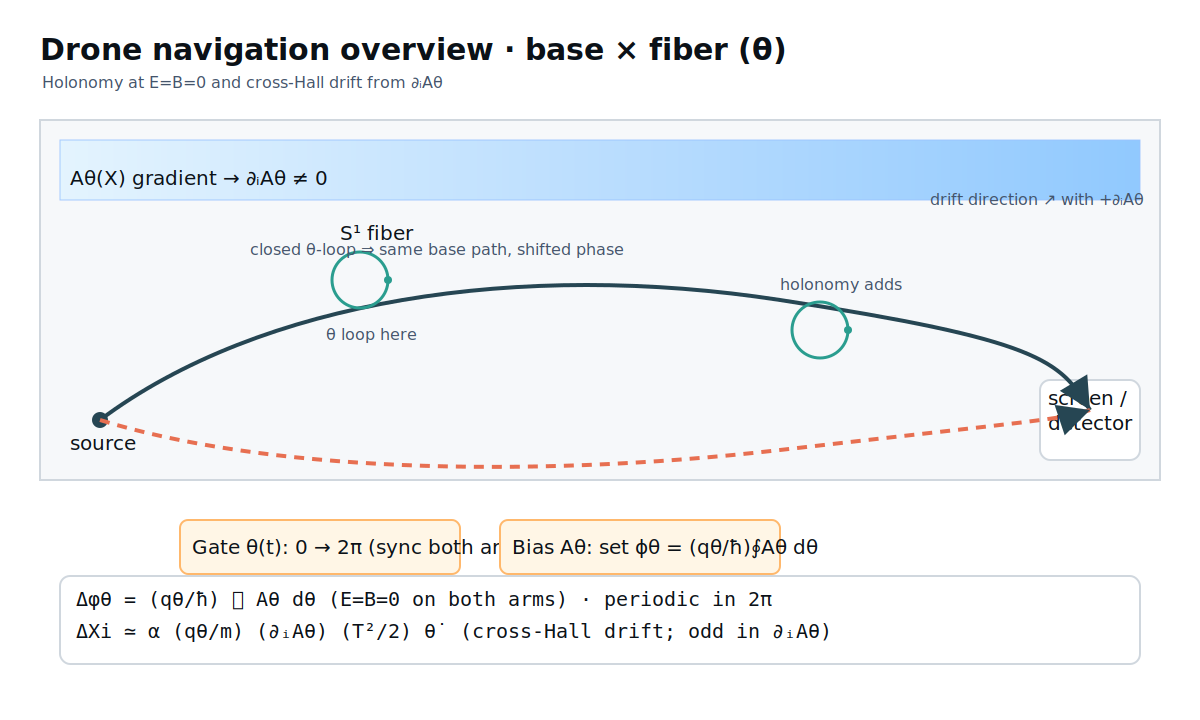
\includegraphics[width=0.75\linewidth]{drone_nav_overview.png}
	\caption{Drone navigation analogy: base motion (drone) with an internal $\theta$ dial (orange). Closing a loop on the dial leaves a transport phase $\hol$ visible at $E=B=0$ along both arms; blue arrows illustrate cross-Hall drifts when $\partial_\mu A_\theta\neq 0$.\label{fig:drone-analogy}}
\end{figure}

Pointers: lab loop-phase readout (\cref{sec:theta-ab}), sidebands as an inertia gauge (\cref{sec:sidebands}), unified range (\cref{sec:unified-force}), and bounce/WDW barrier (\cref{sec:cosmology}).
